\documentclass{article}
\usepackage{spconf_ICME,amsmath,epsfig,fancyhdr}
\setlength{\paperwidth}{215.9mm} \setlength{\hoffset}{-9.7mm}
\setlength{\oddsidemargin}{0mm} \setlength{\textwidth}{184.3mm}
\setlength{\columnsep}{6.3mm} \setlength{\marginparsep}{0mm}
\setlength{\marginparwidth}{0mm} \setlength{\paperheight}{279.4mm}
\setlength{\voffset}{-7.4mm} \setlength{\topmargin}{0mm}
\setlength{\headheight}{0mm} \setlength{\headsep}{0mm}
\setlength{\topskip}{0mm} \setlength{\textheight}{235.2mm}
\setlength{\footskip}{12.4mm} \setlength{\parindent}{1pc}

\ICMEfinalcopy % *** Uncomment this line for the final submission

\def\ICMEPaperID{} % *** Enter the ICME Paper ID here
\def\httilde{\mbox{\tt\raisebox{-.5ex}{\symbol{126}}}}

\ifICMEfinal\pagestyle{empty}\fi

\begin{document}\sloppy

\title{STEREOSCOPIC DEPTH MAPPING}
\name{Eric Henderson, Nicholas Kamper, Laura Moss, James Savage}
\address{Rose-Hulman Institute of Technology\\
Terre Haute, Indiana}

\maketitle
\thispagestyle{fancy} \fancyhead{} \lhead{}
\renewcommand{\headrulewidth}{0pt}
\renewcommand{\footrulewidth}{0pt}

\begin{abstract}
There are many ways to implement depth mapping for 3D vision purposes -- the two primary methods being light-based and stereoscopic. We discuss an implementation of automated stereoscopic depth mapping, including automatic  corresponding point matching using corner detection and window-based feature matching. Using the matched points, we then use the distance between the matched points to determine the distance of the object from the camera. Finally, we display this depth information using a heat map. Overall, we found our implementation to be reasonably accurate, comparable to other stereoscopic depth mapping implementations. Our point matcher was also reasonably accurate, with a few false matches. 
\end{abstract}
\begin{keywords}
stereoscopic vision,depth mapping, stereo vision
\end{keywords}

\section{Introduction}
\label{sec:intro}
Our project implements automated stereoscopic depth mapping in MATLAB.  We take a pair of stereoscopic images, captured at the same time by identical cameras whose backplanes are coplanar, and produce a depth map of relative distances. We then display this depth map in the form of a heat map.  Our general approach was to first obtain so-called interesting points in both images in order to obtain a subset of the image with easily identifiable features.  Then we use feature information from these points to locate corresponding points in the other image. Based on how much each point has shifted, we produce a depth map. In our current version, the depth map is limited to the points that are matched between the two images instead of a full mapping of regions.


\section{Literature Review}
\label{sec:litreview}
\subsection{Hannah, Marsha Jo. ``Digital Stereo Image Matching Techniques.'' International Society for Photogrammetry and Remote Sensing, July 1988.}

\subsubsection{Summary}
In this paper, Hannah presents an overview of various point matching algorithms that can be used to find corresponding pairs of points in stereographic images. 

Hannah describes the algorithms in several classes, including area-based measures that match correlations in patches of the images, edge-based measures that match linear features, global optimization algorithms that can find all corresponding points simultaneously, and feature extractor-based measures that can match single points in images. Hannah primarily describes an area-based algorithm developed at SRI. This algorithm uses iterative refinement and backtracking to improve their results. 

Finally, Hannah describes the performance of the SRI point matching algorithm on a set of test data provided by the ISPRS, stating that for natural scenes, the SRI algorithm performs well. However, the SRI algorithm performed rather poorly on an image of the Olympia dome, not producing any matches. Hannah explains that this is the result of the SRI algorithm being tuned for natural scenes with significant amount of variation and texture and not for the ``bland faces of cultural objects.''

\subsubsection{Applicability}
In our given problem, there are two main subproblems: determining corresponding points in a pair of stereo images and using depth and image information to determine 3D faces of objects. Given that these algorithms are specifically designed for point matching in stereo images, these algorithms should be reasonably suited for use in determining corresponding points. This paper provided the inspiration for our main approach to point matching in that we tried to use the patch correlation as described in the SRI algorithm.

\subsubsection{Issues}
One of the issues with using this paper for our project was the lack of implementation-level detail in the paper. It was difficult to produce a working implementation of the SRI algorithm solely from the limited detail given in the paper. However, there are other papers where the SRI algorithm is described in more depth, such as Hannah's ``Description of SRI's Baseline Stereo System,'' published by SRI and DARPA in October 1984. 

In addition, The SRI algorithm's poor performance on surfaces that were not highly textured was a problem for our algorithm as well, especially if our depth mapping is to be applied in a consumer setting where customers would be expecting the product to work no matter the level of texture of the scene. 


\subsection{Hannah, Marsha Jo. ``Technical Note 342 - Description of SRI's Baseline Stereo System.'' Defense Advanced Research Projects Agency, October 1984. }

\subsubsection{Summary}
In this paper, Hannah presents an area-based point matching algorithm used by SRI as part of a system for doing 3D reconstructions from stereoscopic images. This paper provides much of the implementation detail missing in the other paper by Hannah, Digital Stereo Image Matching Techniques. 

The algorithm is split into two primary steps: preliminary matching and anchored matching. The choice of preliminary matching techniques depend on whether we have the camera parameters, such as the focal length and the principal point. Since we do not want to take the time to calculate the camera parameters, the HMATCH or C2MODEL algorithms devised in the SRI algorithm would work sufficiently. 

Once a set of preliminary corresponding points are selected, these points are then used as ``anchors'' for matching corresponding pairs of points in the near vicinity.  

\subsubsection{Applicability}
As mentioned in the previous literature review for Hannah's Digital Stereo Image Matching Techniques, the SRI algorithm provided the main inspiration for our algorithm, at least at first.  It describes using a outward spiral iteration technique, which we used as one of our approaches before attempting to just map interesting points to one another (as this paper warned against, because of the possibility that an interesting point algorithm may not find the same points in each image).

\subsubsection{Issues}
While the information in this paper resolved some of the concerns with the detail needed for implementation, the SRI algorithm ended up having problems with accuracy on scenes that are sparsely textured. 

\subsection{Thompson, Clark. ``Depth Perception in Stereo Computer Vision.'' Stanford Artificial Intelligence Laboratory, October 1975.}

\subsubsection{Summary}
This paper describes a complete process for the determination of points and depths in two stereo images, including camera setups and algorithms for the computation of matching points in the images. The paper builds on the research of several other sources, offering refinements to their techniques to provide better accuracy for point matching. It also discusses solutions to several of the problems associated with any depth perception algorithms, including how to overcome lens and perspective distortions.

\subsubsection{Applicability}
The work discussed in this paper strongly resembled expected subproblems of our project, including the identification of points and point pairs in two stereo images. This work provided a good foundation for us to start with, although we were not able to take our project further by matching faces in stereo images.

\subsubsection{Issues}
Many issues with the depth perception are listed by the author, and had not yet been solved at the time of writing. Of particular note are problems caused by repeated features in images, which can cause issues in determining proper alignment for the stereo images. In addition, the perspective of source images can create issues in properly aligning points without taking into account the distortion of one of the two images. It is also discouraging that this paper was published in 1975, as much of of the 'Future Work' listed have probably been solved by now.


\section{Process}
\label{sec:Process}
Our process for stereoscopic depth mapping consists of two components: automatically matching corresponding points in both images and then using the distance between those points to determine relative distance from the cameras. 

\subsection{Point Matching}
To be able to use triangulation, we need pairs of matched points between the two stereoscopic images. To find these matched points, we first need to find ``interesting'' points in each of the images and then try to correspond those points to their corresponding point in the other image. 

In theory, one constraint on the corresponding points is that they must be in the same row -- however, since this is not the perfect world, we must assume that the cameras are not perfectly lined up.Therefore, we decided that a 10 pixel horizontal search band was sufficient to cover any variations in the camera positioning while still limiting the search field quite significantly. 

To find interesting points, we tried two different algorithms: directed variance and corner detection

\subsubsection{Directed Variance}

\subsubsection{Corner Detection}
After realizing that directed variance was not going to yield the type of interesting points that we needed, we began to look for other options for finding points that have enough unique features to them that we can accurately match them to their corresponding points in the other image. 

We needed up on using corner detection for finding our points of interest. Corners are fairly unique in terms of features because they have variance in both directions, meaning that they should be relatively easy to match up to other points. 

Our final point matching algorithm finds a fixed number of corners in both images and then tries to correspond the corners in each image together. The primary logic behind only matching corners to corners is that we can assume that a majority of the corners found in one image will have corresponding corners found in the other image due to the fact that both images are assumed to be taken on identical cameras at the same time while pointed at the same scene.

\subsection{Determining Relative Distances}

\section{Results}
\label{sec:Results}
\subsection{Results of our Corner-based Point Matching}
% Image 1
\begin{figure}[H]\centering
	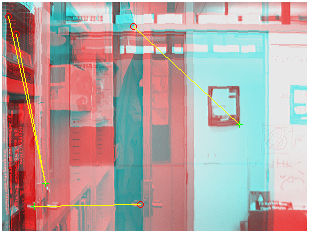
\includegraphics[width=0.8\linewidth]{Images/01_matlab_match.png}
	\caption{Interesting points and matches found using MATLAB's implementation on Image 1.}
	\label{fig:jp-ofc-matlab-match}
\end{figure}

\begin{figure}[H]\centering
	
\includegraphics[width=0.8\linewidth]{Images/01_matlab_depth.png}
	\caption{Depth map using the interesting points and matches using MATLAB's implementation on Image 1.}
	\label{fig:jp-ofc-matlab-depth}
\end{figure}

\begin{figure}[H]\centering
	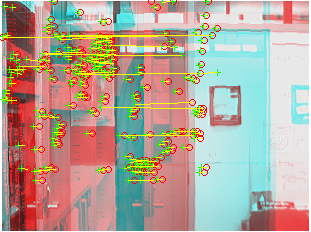
\includegraphics[width=0.8\linewidth]{Images/01_our_match.png}
	\caption{Interesting points and matches using our implementation on Image 1.}
	\label{fig:jp-ofc-ours-match}
\end{figure}

\begin{figure}[H]\centering
	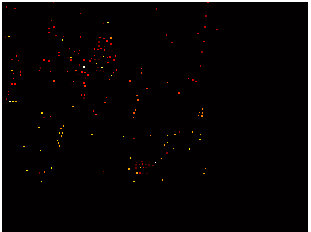
\includegraphics[width=0.8\linewidth]{Images/01_our_depth.png}
	\caption{Depth map using the interesting points and matches using our implementation on Image 1.}
	\label{fig:jp-ofc-ours-depth}
\end{figure}

% Image 2
\begin{figure}[H]\centering
	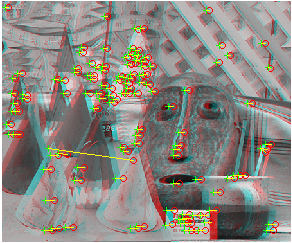
\includegraphics[width=0.8\linewidth]{Images/02_matlab_match.png}
	\caption{Interesting points and matches found using MATLAB's implementation on Image 2.}
	\label{fig:cones-matlab-match}
\end{figure}

\begin{figure}[H]\centering
	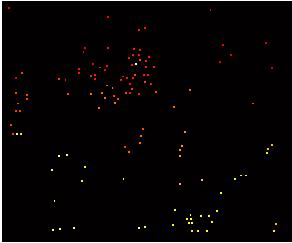
\includegraphics[width=0.8\linewidth]{Images/02_matlab_depth.png}
	\caption{Depth map using the interesting points and matches using MATLAB's implementation on Image 2.}
	\label{fig:cones-matlab-depth}
\end{figure}

\begin{figure}[H]\centering
	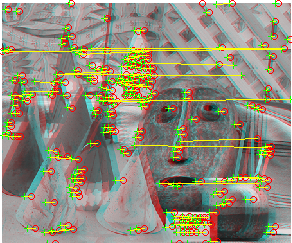
\includegraphics[width=0.8\linewidth]{Images/02_our_match.png}
	\caption{Interesting points and matches using our implementation on Image 2.}
	\label{fig:cones-ours-match}
\end{figure}

\begin{figure}[H]\centering
	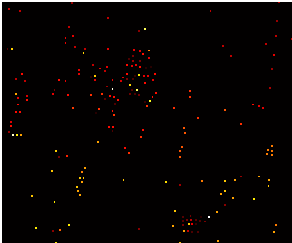
\includegraphics[width=0.8\linewidth]{Images/02_our_depth.png}
	\caption{Depth map using the interesting points and matches using our implementation on Image 2.}
	\label{fig:cones-ours-depth}
\end{figure}

% Image 3
\begin{figure}[H]\centering
	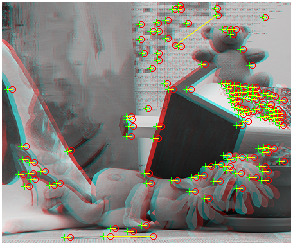
\includegraphics[width=0.8\linewidth]{Images/03_matlab_match.png}
	\caption{Interesting points and matches found using MATLAB's implementation on Image 3.}
	\label{fig:bear-matlab-match}
\end{figure}

\begin{figure}[H]\centering
	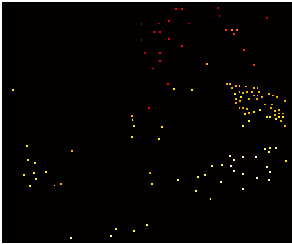
\includegraphics[width=0.8\linewidth]{Images/03_matlab_depth.png}
	\caption{Depth map using the interesting points and matches using MATLAB's implementation on Image 3.}
	\label{fig:bear-matlab-depth}
\end{figure}

\begin{figure}[H]\centering
	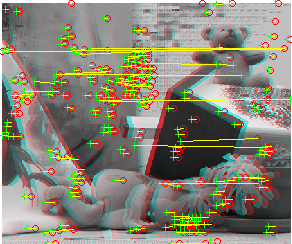
\includegraphics[width=0.8\linewidth]{Images/03_our_match.png}
	\caption{Interesting points and matches using our implementation on Image 3.}
	\label{fig:bear-ours-match}
\end{figure}

\begin{figure}[H]\centering
	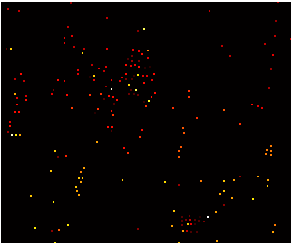
\includegraphics[width=0.8\linewidth]{Images/03_our_depth.png}
	\caption{Depth map using the interesting points and matches using our implementation on Image 3.}
	\label{fig:bear-ours-depth}
\end{figure}

While we had to settle for our fallback goal of creating only a partial depth map, we do believe that our approach showed some merit. Above are shown some examples of our point matching compared with MATLAB's, which uses a 11$\times$11 window as per MATLAB's documentation, and the same depth mapping applied to the results of each set. As you can see in these, our implementation compares reasonably well with MATLAB given the same corner data. This is especially true for the image used in Figures \ref{fig:jp-ofc-matlab-match}-\ref{fig:jp-ofc-ours-depth}, as our algorithm performed exceptionally better than MATLAB, (which actually produced no valid correlations). We assume that this is because of the assumption we make that a match point will lie within a 10-pixel band of its source, allowing us to make more forgiving matches in the case of harsher perspective shifts between the two images.

MATLAB's point correlation did tend to produce smoother depth maps for images with only minor differences however, whereas our implementation introduced substantial noise. This noise is particularly apparent in images like \ref{fig:cones-ours-depth}, with scattered bright spots near the middle. However, the general trend of closer foreground objects toward the bottom images and farther background images toward the top is consistent with what we expect. Our algorithm also had the tendency to make matches that went completely across the image, which we dealt with by discarding outliers above two standard deviations. However, even with this weighting, it simply turned out that these matches were the best that the algorithm could find -- likely a result of being a greedy algorithm and just matching whatever points were left over.  Another possible reason for poor matches in our algorithm, theoretically, is that the corners found in each image may not necessarily be the same.


\section{Conclusion}
\label{sec:conclusion}
Overall, we were satisfied by the results of our algorithm given the time constraints of our project. Given more time, we would've been able to significantly improve our results. 

\subsection{Challenges Encountered}
\label{conclusion:challenges}
We encountered several challenges during the course of this project. 
\subsubsection{Finding Corresponding Points}
We encountered significant amount of difficulty in finding corresponding matching points. Even with the constraint of being able to limit the number of rows to search, our greedy point matching algorithm still encountered difficulty primarily because we were matching corners to corners -- if the corresponding corner wasn't detected by the corner detector, it will correspond the corner with a random corner. 

One way we could resolve the issue of undetected corresponding corners would be to allow unmatched corners. 

\subsubsection{Optimizing MATLAB Code}
We had significant problems with optimizing our algorithms for performance. In general, our algorithm implementations are not fast enough to be able to used in real-time. However, given more time, we would be able to optimize our MATLAB code or rewrite our implementation in native C/C++, potentially using OpenCV. With more time, our goal would be to improve the performance enough that we could handle 5-10fps on a multi-core machine. 

\subsubsection{Varying Accuracy and Camera Limitations}
In some cases, we found that the accuracy of our algorithm ranged from good to abysmal. This isn't a problem specifically with our implementation, but rather with the general principle of stereoscopic depth mapping. For objects that are far away, their corresponding points could potentially map to the same cell on the sensor. Very small changes in distance could also map to the same cell. This would make stereoscopic depth mapping not suitable for use for 3D modeling or other fields requiring a large degree of accuracy. 

\subsubsection{Unknown Camera Parameters}
One way that we could've improved our algorithms would be through the use of information about the camera. For instance, we would be able to obtain the actual distances away from the camera if we knew the field of view angle and distance between the stereo cameras. However, most of the images we used did not contain both pieces of information necessary. 

\section{Challenges Encountered}
\label{conclusion:challenges}
We encountered several challenges during the course of this project. 
\subsection{Finding Corresponding Points}
We encountered a significant amount of difficulty in finding corresponding points. Even with the constraint of being able to limit the number of rows to search, our greedy point matching algorithm still encountered difficulty primarily because we were matching corners to corners -- if the corresponding corner wasn't detected by the corner detector, it would correspond the corner with a random corner. 

One way we could resolve the issue of undetected corresponding corners would be to allow unmatched corners. 

\subsection{Optimizing MATLAB Code}
We had significant problems with optimizing our algorithms for performance. In general, our algorithm implementations are not fast enough to be able to used in real-time. However, given more time, we would be able to optimize our MATLAB code or rewrite our implementation in native C/C++, potentially using OpenCV. With more time, our goal would be to improve the performance enough that we could handle 5-10fps on a multi-core machine. 

\subsection{Varying Accuracy and Camera Limitations}
In some cases, we found that the accuracy of our algorithm ranged from good to abysmal. This isn't a problem specifically with our implementation, but rather with the general principle of stereoscopic depth mapping. For objects that are far away, their corresponding points could potentially map to the same cell on the sensor. Very small changes in distance could also map to the same cell. This would make stereoscopic depth mapping not suitable for use for 3D modeling or other fields requiring a large degree of accuracy. 

\subsection{Unknown Camera Parameters}
One way that we could have improved our algorithms would be through the use of information about the camera. For instance, we would be able to obtain the actual distances away from the camera if we knew the field of view angle and distance between the stereo cameras. However, most of the images we used did not contain both pieces of information necessary.

\section{Future Work}
\label{sec:future}
We have several directions that we would have liked to explored given the time. 

\subsection{Improved Point Matching}
Our current point matching algorithm, while reasonably accurate, could still use some improvements. One potential idea is to incorporate multiple sources for the interesting points, such as using raw edgels. In addition, we would also like to explore using features in addition to RGB color distance for comparing regions. One such feature might be to compare the partial derivatives of the image, essentially matching the edges in the two windows. 

One suggestion that we received during our presentation was the possibility of using motion algorithms to help determine corresponding points between the two images. If we know the amount of motion that a particular object takes, we can search a small region around where we would expect the object to be in the other image to determine corresponding points. Using this in conjunction with our corner-based interesting point detection would allow us to map significantly more points, resulting in more depth data for an image. 

Finally, a way to significantly improve our point matching would be to gather intrinsic camera parameters, either by an explicit camera calibration step or using the \textit{C2MODEL} algorithm suggested in the SRI paper, and to find the epipolar line in the corresponding image. With the epipolar line, we would know that the corresponding point would lie somewhere on that line. This would reduce our search from a 2-dimensional search to a simple 1-dimensional search.

\subsection{Regions of Depth}
Instead of getting the depth of single points, one potential improvement would be to get the depth of entire planes in the image, such as the face of a box. This would allow us to produce a full depth map of a scene for every point in the scene.

One potential way of implementing this would be to use the anchored point matching algorithm, such as \textit{GMATCH}, suggested in the SRI paper for getting additional point matches around the interest points. In theory, we could perform anchored point matching to get corresponding points for all of the overlapping points within the image. From there, we can use edge detection to determine the boundaries of plane faces and merge those distances into a smooth depth gradient rather than a collection of depths of points. 

With this implemented, our project could be potentially useful for creating 3D models of scenes using just stereoscopic data.

\subsection{Absolute Distances}
One of the limitations of our current implementation is that we cannot determine absolute distances away from the camera (e.g., saying that point X is 15 feet away from the camera). One way we could potentially get this information would be to calibrate our implementation using known distances (e.g., calibrate the setup by saying that object X is 5 feet away and object Y is 10 feet away) and using that information to determine the field of view angle for the camera. 

One potential limitation of this approach is that some cameras have asymmetrical field of view angles, viewing the image in an oval rather than square. As such, we would need to account for this by taking multiple measurements. Another approach would be to simply use cameras where we know the field of view angles.




\end{document}
